\apendice{Plan de Proyecto Software}

\section{Introducción}
En este apartado de la documentación de los anexos se pretende exponer de manera cronológica como ha ido evolucionando el desarrollo del estudio realizado.

Durante la maduración del mismo se ha empleado la metodología \textit{Scrum} para dividir cada fase del proyecto en \textit{sprints}, dentro de cada cuál se incluye una planificación, un desarrollo y una revisión en forma de reunión del mismo.

A lo largo del desarrollo del estudio, se han ido anotando todas las tareas solicitadas para cada sprint en el \href{https://github.com/hds1001/Estudio-y-configuracion-de-un-sistema-ELK}{repositorio} GitHub del proyecto, por lo que en este apartado se hará un desglose de cada tarea involucrada.

Además de todo lo mencionado anteriormente, también se va a estudiar la viabilidad del proyecto, tanto económica, como legal.

\paragraph{}
\paragraph{}
\paragraph{}
\paragraph{}
\paragraph{}


\section{Planificación temporal}

\subsection{Sprint 1 (15/02 - 17/03)}
\subsubsection{Planificación}
Tras una primera toma de contacto entre los miembros del estudio, se acordó que inicialmente se comenzaría con un trabajo de investigación sobre el funcionamiento de cada componente de un sistema basado en ELK, así como la instalación de los mismos y prueba de que se ejecutaban correctamente.

También se encomendó la tarea de crear el repositorio GitHub del estudio, en el que se irían actualizando, a medida que se avanzaba las \textit{issues} del proyecto.

\subsubsection{Issues}
\begin{itemize}
    \item \textbf{Investigación e instalación de Kibana}
    \item \textbf{Investigación e instalación de ElasticSearch}
    \item \textbf{Investigación e instalación de Logstash}
    \item \textbf{Configuración del repositorio GitHub}
    \item \textbf{Inicio documentación de la memoria}

    \end{itemize}

\subsubsection{Desarrollo}
En este primer mes se investigó a través de las fuentes principales de información de cada programa su instalación y uso básico de cara a probar con pruebas lo que ofrecían. En primer lugar ElasticSearch no opuso grandes dificultades, puesto que posee una extensa documentación, y su ejecución fue relativamente sencilla, cosa que no ocurrió con Logstash, ya que su comprensión era más compleja y requería de conocimientos más elevados que para las otros dos componentes. Por último, en Kibana fue en el que más profundizo en este sprint, puesto que era el programa más intuitivo que más posibilidades y complementos ofrecía.

También se hizo énfasis en analizar programas alternativos a estos comparando las ventajas e inconvenientes frente a Elastic, Logstash y Kibana.

\subsubsection{Revisión}
En la segunda reunión se compartieron los resultados encontrados y por parte del tutor el programa que más interés desperto fue Logstash, puesto que las opciones que ofrecía erán las más interesantes de estudiar, cimentando así las bases del segundo sprint que comenzaría inmediatamente después.

\subsection{Sprint 2 (18/03 - 03/04)}
\subsubsection{Planificación}
En esta segunda fase del proyecto, una vez conocidas las características básicas de los componentes y como se relacionan entre sí, se creyó conveniente profundizar en las posibilidades de filtrado que ofrece Logstash, sabiendo diferenciar qué se puede y qué no se puede hacer.

También se empezó a mencionar la idea de aplicar tanto Machine Learning como MapReduce en algún momento del proceso a los datos, por lo que se encomendó el comienzo de la investigación de ambos temas.

\subsubsection{Issues}
\begin{itemize}
    \item \textbf{Comenzar con la documentación de la memoria en LaTeX}
    \item \textbf{Investigar sobre la funcionalidad de Machine Learning en Elastic}
    \item \textbf{Investigar funcionamiento filtrado Logstash}
    \item \textbf{Investigar desarrollo con plugins en ElasticSearch}
    \item \textbf{Investigar posible integración con Python para el tratamiento de datos}
    \item \textbf{Investigar desarrollo con Docker y como integrarlo}
    \item \textbf{Investigar funcionamiento MapReduce en Logstash}
    \item \textbf{Investigar funcionamiento MapReduce en ElasticSearch}
    \item \textbf{Investigar funcionamiento MapReduce en Kibana}
    \item \textbf{Probar filtrado en Logstash: sumas, agrupamientos, discretizar columna numérica}
    \item \textbf{Continuar con documentación en Overleaf}
    \item \textbf{Familiarización con librería SKLearn en cuanto a clasificación, regresión, clustering y PCA}
\end{itemize}

\subsubsection{Desarrollo}
Se investigó la posibilidad que ofrecía el plugin de Machine Learning que ofrece ElasticSearch, cuyas funciones gratuitas son limitadas, y las más interesantes son de pago. Por parte del tutor, se ofreció una fuente de información para poder aplicar funciones de Machine Learning de manera gratuita a fuentes de datos, \textit{Scikit-Learn}, de manera que durante este tiempo el estudio se enfocó en comprender el funcionamiento de esta librería, y de qué manera la podíamos acoplar en el sistema ELK.

Por otro lado, indagar en las funciones avanzadas de Logstash, fue costoso, puesto que la información presente en internet era escasa y la mayoría antigua, por lo que las pruebas con este programa fueron un claro ensayo y error hasta dar con la tecla. Se profundizo en las operaciones de filtrado, agrupamientos básicos y discretizaciones en el apartado \textit{filter} de el archivo de configuración.

\subsubsection{Revisión}
En la tercera y cuarta reunión entre los miembros se discutió sobre qué filtros erán más interesantes de aplicar, el orden que debían seguir los datos a lo largo de todo el proceso ETL, y cómo se podían integrar los resultados obtenidos por las funciones de \textit{Scikit-Learn} en Elastic para su posterior exposición en Kibana. Concluyendo así el segundo sprint del proyecto y abriendo temas para la tercera fase.

\paragraph{}
\paragraph{}
\paragraph{}
\paragraph{}
\paragraph{}

\subsection{Sprint 3 (04/04  - 20/04)}
\subsubsection{Planificación}
Y así entramos en la tercera etapa del estudio, en la que se plantearon tareas a realizar como la carga con éxito de los datos del script del Iris en Kibana, continuar explorando los filtros de Logstash, y abordar el tema los \textit{streamings} de datos, que aún no estaba desarrollado en este momento del estudio.

Otro punto a destacar como importante de cara a realizar en esta fase, es el de conseguir realizar de manera eficiente y útil  MapReduce en Logstash.

\subsubsection{Issues}
\begin{itemize}
    \item \textbf{Cargar datos Iris en Kibana}
    \item \textbf{Explorar más posibilidades de agrupamiento en Logstash con máximos, medias, etc.}
    \item \textbf{Probar Data Streams: los que se puede y no (funcionamiento, campos, etc.)} 
    \item \textbf{Comparar MapReduce en Kibana con Logstash}
    \item \textbf{Probar Data Streams: los que se puede y no (funcionamiento, campos, etc.)}
\end{itemize}

\subsubsection{Desarrollo}
Por un lado, gracias a los foros presentes en las páginas oficiales tanto de Elastic como de \textit{Scikit-Learn}, se consiguió combinar los dos, de manera que el tráfico de información entre ambos fuera fluido y exitoso. Esto se hizo tras realizarle unas modificaciones al script tanto en la forma en la que ingestaba los datos, como en la de como se exportaban los mismos, y hacia donde.

El tema de los \textit{data streams} siguió sin avanzar, puesto que no se encontraba de qué manera se podía implementar esta forma de ingesta de datos en el sistema ELK. 

Y trás darle unas cuantas vueltas, se llegó a la conclusión de que la manera de realizar el MapReduce en Logstash era con su función \textit{aggregate}.

\subsubsection{Revisión}
Así se cubrió lo relacionado con \textit{Scikit-Learn} de manera parcial y cubriendo la tarea encomendada, mientras que los \textit{streamings} de datos en vivo seguía en el aire y sin saber muy bien hacia donde seguir tirando.

\subsection{Sprint 4 (22/04 - 30/04)}
\subsubsection{Planificación}
Para este cuarto sprint, se vió que el tema de los \textit{data streams} había que terminarlo, por lo que se le dió máxima relevancia a este, de manera que se pudieran mandar datos en tiempo real a Elastic de manera que se les aplicara un filtrado con Logstash y pudieran ser expuestos en Kibana.

\subsubsection{Issues}
\begin{itemize}
        \item \textbf{Probar funcionamiento Data Streams}   
    \item \textbf{Investigar funcionamiento WebSocket en ELK}
        \item \textbf{Conectar WebSocket con Logstash}
\end{itemize}

\subsubsection{Desarrollo}
Esto se logró gracias a las herramientas \textit{WebSocket}, la cuál permitio poder conectarnos a una fuente de datos, \textit{Finnhub}, que mandara los datos tanto a Elastic como a Logstash, y esos datos fueran depurados para ser mostrados en un \textit{dashboard} de Kibana. Esto se consiguió gracias a un \href{https://github.com/ColinEberhardt/awesome-public-streaming-datasets}{repositorio} público de GitHub que ofrecía diferentes maneras de interactuar con datos en vivo.

De manera paralela a los \textit{WebSockets}, se trabajó con una herramienta del ecosistemas Elastic llamada \textit{Filebeat}, la cuál ofrecía cubir la necesidad de poder mandar datos en \textit{streaming} hacia Elastic o Logstash, pero al ver que la alternativa encontrada era más eficiente y ofrecía más posibilidades, se optó por los \textit{WebSockets}.

\subsubsection{Revisión}
En la sexta reunión de los miembros se mostró tranquilidad al ver que gran parte de los problemas presentes habían sido solventados y que se comprendía de que manera se podían implementar \textit{data streams} en el sistema ELK.

Con esto, se empezó a plantear la posibilidad de empezar a preparar los escenarios finales junto con la documentación de el funcionamiento de cada uno.

\subsection{Sprint 5 (31/04 - 06/05)}
\subsubsection{Planificación}
Por lo que en la séptima reunión se hizo retrospectiva de lo que se tenía hasta el momento, y se decidió que el tema de las transformaciones de datos en Logstash aún no estaba en un buen punto, por lo que en este sprint se centró el tiempo en cerrar todo esto.

También se dió enfásis a la idea del \textit{Edge Computing}, y como podía ser relevante aplicarlo en el estudio.

\subsubsection{Issues}
\begin{itemize} 
    \item \textbf{Estudiar posibilidad hacer MapReduce del data stream en Logstash}  
    \item \textbf{Investigar funcionamiento MapReduce en Kibana}    
    \item \textbf{Investigar sobre el Edge Computing y como funciona} 
\end{itemize}

\subsubsection{Desarrollo}
Finalmente se terminó de cerrar todo lo relacionado con los filtrados en Logstash al aplicar distintas funciones a una fuente de datos. Funciones como:
\begin{itemize}
    \item Borrar campos vacíos
    \item Transformación de tipos
    \item Operaciones con distintos campos
\end{itemize}

Por otra parte, hubo un trabajo de investigación sobre \textit{Edge Computing} de cara a poder documentarlo en la memoria, y se comprendió la idea que se le asociaba.

\subsubsection{Revisión}
Así se concluyó esta quinta fase, dando por sentados todos los escenarios que iban a estar presentes en la documentación técnica, y se comenzó a plantear la idea de la preparación e ilustración de los mismos.

\subsection{Sprint 6 (07/05 - 16/05)}
\subsubsection{Planificación}
Llegando a esta sexta etapa ya se empezaba a divisar el final en el horizonte y se encomendó la tarea de ilustrar y preparar minuciosamente cada escenario tratado de manera que la documentación de los mismos fuera más sencilla.

\subsubsection{Issues}
\begin{itemize}
    \item \textbf{Estudiar caso importar directamente el fichero en Elastic}
    \item \textbf{Estudiar caso importar el fichero desde Logstash}
    \item \textbf{Estudiar caso importar un DataSet (Iris)}
    \item \textbf{Estudiar caso importar a través de WebSocket a Elastic}
    \item \textbf{Estudiar caso importar a través de un WebSocket con Logstash}

    \end{itemize}
    

\subsubsection{Desarrollo}
Durante este tiempo se trabajó en preparar todos los directorios con la información relevante de cada escenario, así como ilustrar los \textit{dashboards} finales obtenidos en cada uno.

Se empezó a documentar en \textit{Overleaf}  la memoria del estudio de manera básica para ir teniendo un punto de partida.

\subsubsection{Revisión}
Tras la novena reunión de miembros se empezaron a realizar correcciones a la memoria y reestructuraciones a los escenarios de manera que las ideas presentadas fueran más claras y concisas.

\subsection{Sprint 7 (17/05 - 10/06)}
\subsubsection{Planificación}
En esta séptima etapa se continuó con el plan pensado para la anterior de seguir documentando los escenarios y los diferentes apartados de la memoria técina del estudio.

\subsubsection{Issues}
\begin{itemize}


    \item \textbf{Investigar sobre el caso de Edge Computing y cómo funciona}
    \item \textbf{Continuar desarrollo de escenarios}



\end{itemize}

\subsubsection{Desarrollo}
Por lo que todo este tiempo se dedicó a realizar modificaciones y continuar agregando información a la memoria corrigiendo la estructura y los contenidos de cada apartado de manera que fuerán más acordes a un trabajo científico.

\subsubsection{Revisión}
Siguiendo la pauta de la anterior reunión las reuniones octava y novena estuvieron enfocadas a seguir mejorando el trabajo realizado en al documentación.

\subsection{Sprint 8 (11/06 - 10/07)}
\subsubsection{Planificación}
Tras una serie de revisiones tanto de la documentación de los anexos como de la memoria, se han planteado diversas mejoras en ambos por parte del tutor. También se ha mencionado el modificar el script en el que se aplica Machine Learning, de manera que los datos se carguen desde Elastic y una vez procesados sean devueltos. Para terminar se encomendó la tarea de realizar videos explicativos del proyecto, el pulido final del repositorio y la creación de una máquina virtual que contenga todo lo relacionado con el proyecto.

\subsubsection{Issues}
\begin{itemize}


    \item \textbf{Documentación de la memoria}
    \item \textbf{Documentación de los anexos}



\end{itemize}

\subsubsection{Desarrollo}
Se dedicó todo el último mes a pulir detalles en la documentación de manera satisfactoria mediante una serie de revisiones. Se consiguió modificar la fuente de ingesta del script de Machine Learning con éxito, y se trabajó en todo lo mencionado para que la entrega del proyecto se pudiera hacer en fecha.

\subsubsection{Revisión}
Tras una última revisión de los contenidos, ambas partes quedaron satisfechas con el resultado y se acordó que esa era el producto final a entregar.

\paragraph{}
\paragraph{}
\paragraph{}
\paragraph{}
\paragraph{}
\paragraph{}
\paragraph{}
\paragraph{}
\paragraph{}
\paragraph{}
\paragraph{}
\paragraph{}

\section{Estudio de viabilidad}

\subsection{Viabilidad económica}
A lo largo de este estudio se ha empleado una versión gratuita de Elastic, en la cual, por ejemplo, el plugin que habilita la función Machine Learning, está bloqueado. Elastic ofrece esta y más funciones en sus diferentes niveles de suscripción:

\begin{enumerate}
    \item \textbf{Basic (Gratis)}
\begin{itemize}
        \item Ofrece un amplio mercado de plugins y de características limitadas, entre las cuales no se encuentra la de aplicar Machine Learning a los índices de datos. Se ofrecen integraciones para transmitir logs, métricas, rastreos, contenido y más desde diferentes fuentes. 
    \end{itemize}
    \item \textbf{Gold (109 doláres al mes)}
    \begin{itemize}
        \item Ofrece características adicionales de seguridad, monitoreo de datos y algunas funciones de Machine Learning.
    \end{itemize}
    \item \textbf{Platinum (125 doláres al mes)}
    \begin{itemize}
        \item Ofrece todas las características del nivel Gold, además de acceso completo a las capacidades de Machine Learning, alertas avanzadas, y soporte premium.
    \end{itemize}
    \item \textbf{Enterprise (175 dólares al mes)}
    \begin{itemize}
        \item Ofrece todas las características del nivel Platinum, con funcionalidades adicionales de administración de los datos y un mejor soporte.
    \end{itemize}
\end{enumerate}

Sklearn no supone coste alguno puesto que es una herramienta de código abierto. El \textit{hardware} empleado ha sido un ordenador de unos 500€.

Suponiendo que en este trabajo se han invertido unas 600 horas de trabajo a lo largo de 5 meses, que son aproximadamente 21 semanas. Asignando unas 28 horas de carga de trabajo semanal, y teniendo en cuenta que el salario del alumno será de 18€/hora, se obtiene un salario bruto de entorno a 2000€/mes. Este salario una vez se le aplica las deducciones por impuestos indicadas en la \href{https://www.seg-social.es/wps/portal/wss/internet/Trabajadores/CotizacionRecaudacionTrabajadores/36537}{página de la seguridad social} (ver figuras \ref{fig:coti1} y \ref{fig:coti2}).

\begin{figure}
    \centering
    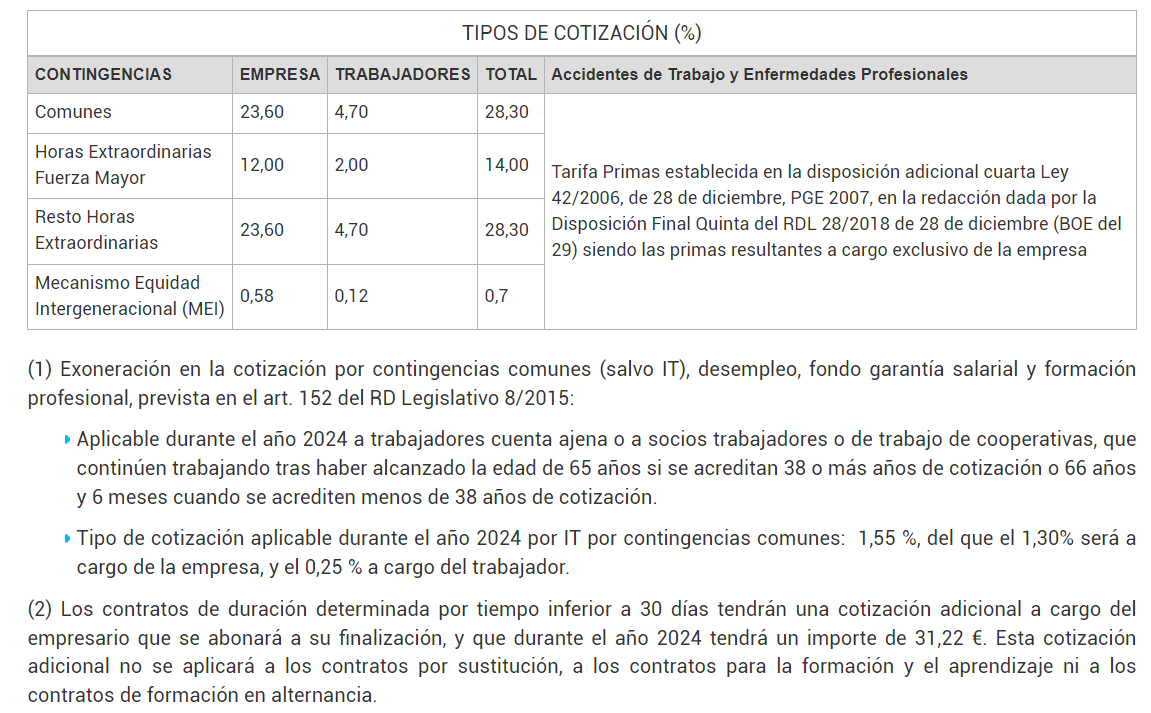
\includegraphics[width=1\linewidth]{img/cotizacion1.png}
    \caption{Tipos de cotización en el régimen general de la Seguridad Social.}
    \label{fig:coti1}
\end{figure}

\begin{figure}
    \centering
    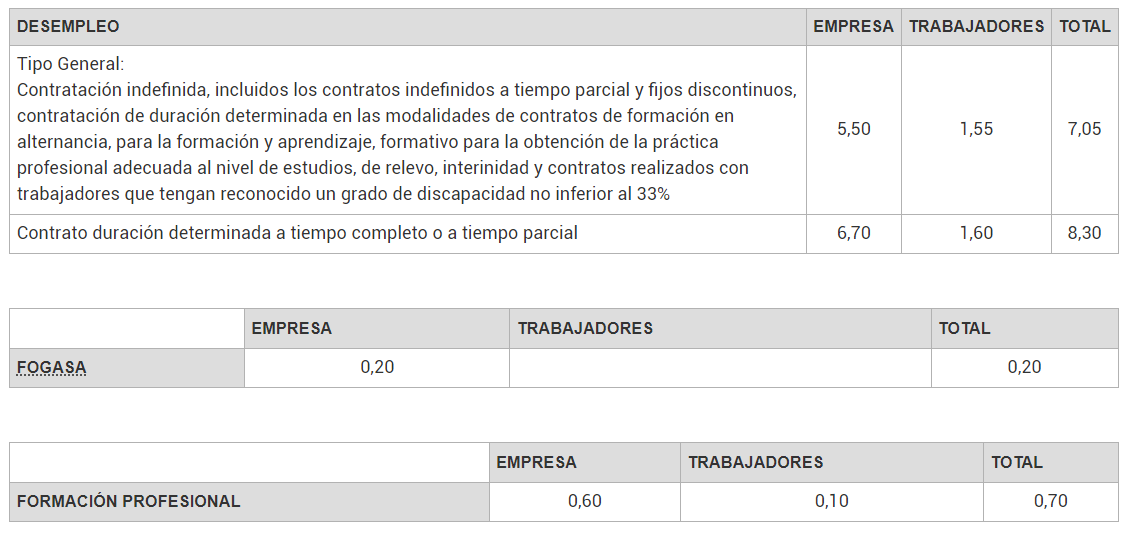
\includegraphics[width=1\linewidth]{img/cotizacion2.png}
    \caption{Más tipos de cotización en el régimen general de la Seguridad Social.}
    \label{fig:coti2}
\end{figure}

Los impuestos supondrán un 23,6 por ciento del sueldo en concepto de contingencias, un 5,5 por ciento en concepto de desempleo, un 0,2 en concepto de FOGASA y un 0,6 en concepto de formación profesional por parte de la empresa. Aplicando todos estos porcentajes el sueldo real del alumno alcanzaría la cifra de 2853€/mes.

Además del alumno también hay que tener en cuenta que se trabaja con dos profesores cumpliendo el rol de tutores. Siendo el salario mensual de 38€, y suponiendo que que trabajan 2 horas por semana, el sueldo bruto de los dos profesores será de 608€/mes, que con la aplicación de impuestos se queda en 867€/mes reales.

Una vez se tienen los datos sobre la mesa, el gasto mensual que supone el proyecto en total es de 3461€, que multiplicado por los 5 meses de duración del trabajo se quedan en 17305€ de coste total.

\subsection{Viabilidad legal}
Un sistema ELK usa principalmente dos tipos de licencias: 
\begin{itemize}
    \item La Licencia de Apache 2.0 para versiones anteriores a la 7.11. Esta licencia permite un uso comercial, de distribución, modificación y patente incluyendo un aviso de \textit{copyright} y de licencia.
    \item La Licencia Elastic para versiones a partir de la 7.11. Esta también ofrece licencias básicas gratuitas y comerciales para acceso a funciones avanzadas y soporte técnico.
    \item Sklearn posee una licencia BSD 3-Clause que otorga permisos comerciales, de distribución y modificación incluyendo un aviso de \textit{copyright} y de licencia.
\end{itemize}

